

\section{MNIST results}


\subsection{GAN vs CGAN}

It is important to notice that CGAN architecture works much better than the original GAN architecture on MNIST (Fig 6.1 and 6.2)


\begin{figure}[!tbp]
  \centering
  \begin{minipage}[b]{0.45\textwidth}
    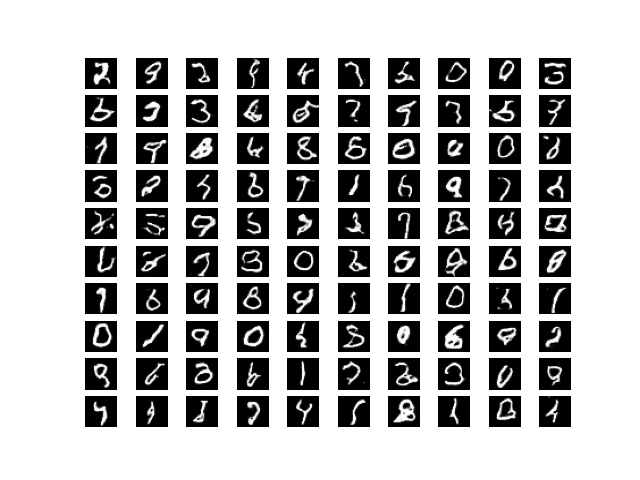
\includegraphics[width=\textwidth]{mnist_unconditional_example}
    \caption{Generated MNIST data by GAN}
  \end{minipage}
  \hfill
  \begin{minipage}[b]{0.45\textwidth}
    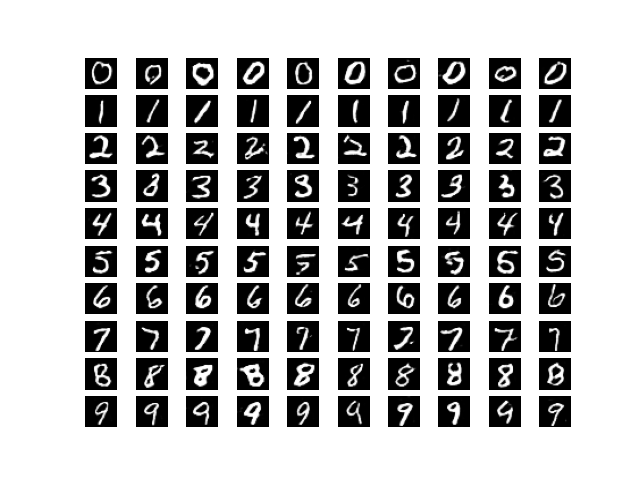
\includegraphics[width=\textwidth]{mnist_conditional_all}
    \caption{Generated MNIST data by CGAN}
  \end{minipage}
\end{figure}


This phenomena can be understood just by thinking on the process of handwriting: 

Conditioning the 'main attributes' of the generated handwriting should be based on the text. This how humans write. The content and the style are separated. Giving the model this ability produces much better results, and it also can be though as a tool to extract meaningful insights (though not implemented in this project).


\subsubsection{Disentanglement of style and content}
The CGAN model consists an additional layer to the generator structure - an embedding layer from the labels space to the pixels space.
The embedded layer learns the "content", and the latent space variations control the different style characteristics of the digit. 

We can find a confirmation to that claim be looking at figure 6.3 - the same noise seed generates all digits on the same row, and all of these samples seem to share the same style (width and orientation are the most obvious ones from the 1st and 9th rows).


\begin{figure}[h]
\centering
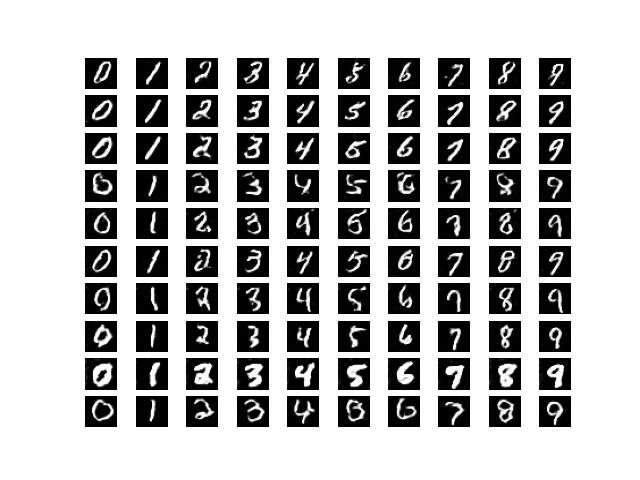
\includegraphics[scale=0.8]{mnist_conditional_same_z}
\caption{Generated MNIST data by CGAN, each row is generated from the same seed in latent space}
\label{fig:x cubed graph}
\end{figure}


Notice that the same qualitative insight can be inferred from Graves work (Generating Sequences With RNNs). 
The conditioned samples (those who are generated from text, and not just by sampling from the model) look much more realistic, beside the fact that they actually form meaningful words. Note that there seems to be real letters in the unconditional sample, but they are not accurate as in the conditional one.


\begin{figure}[h]
\centering
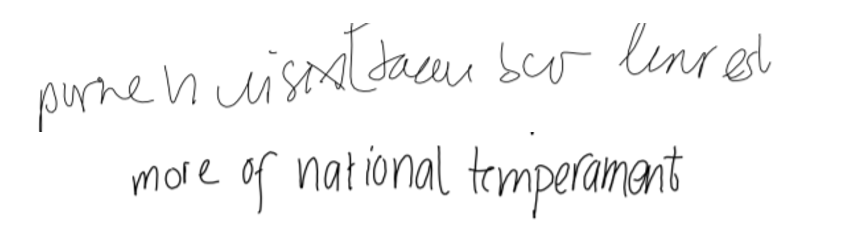
\includegraphics[scale=0.8]{rnn-unconditional_vs_conditional}
\caption{unconditional (first row) vs conditional sampling (second row) in Graves work on IAM online Data}
\label{fig:x cubed graph}
\end{figure}


\subsubsection{Directions in latent space}


By exploring the directions in the latent space, we can visualize the changes in style versus the changes in the latent space (linearly).
In the vanilla GAN, the changes in the latent space seems to modify the shapes of the output digits, and not only what we refer to as their 'styles'.



\begin{figure}[h]
\centering
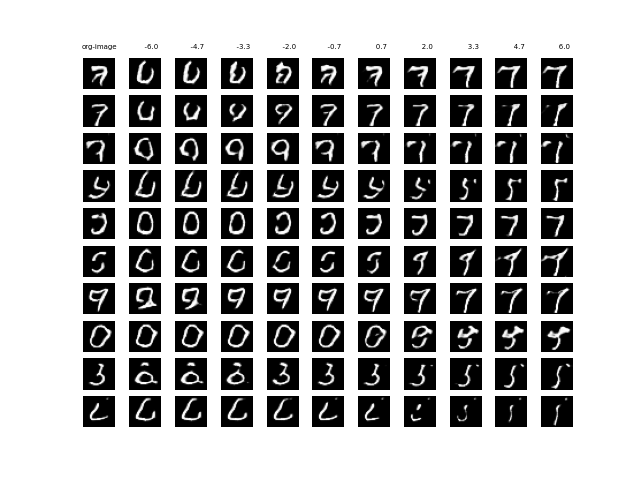
\includegraphics[scale=1]{gan_d1}
\caption{Discovered direction of GAN on MNIST}
\label{fig:x cubed graph}
\end{figure}


\begin{figure}[h]
\centering
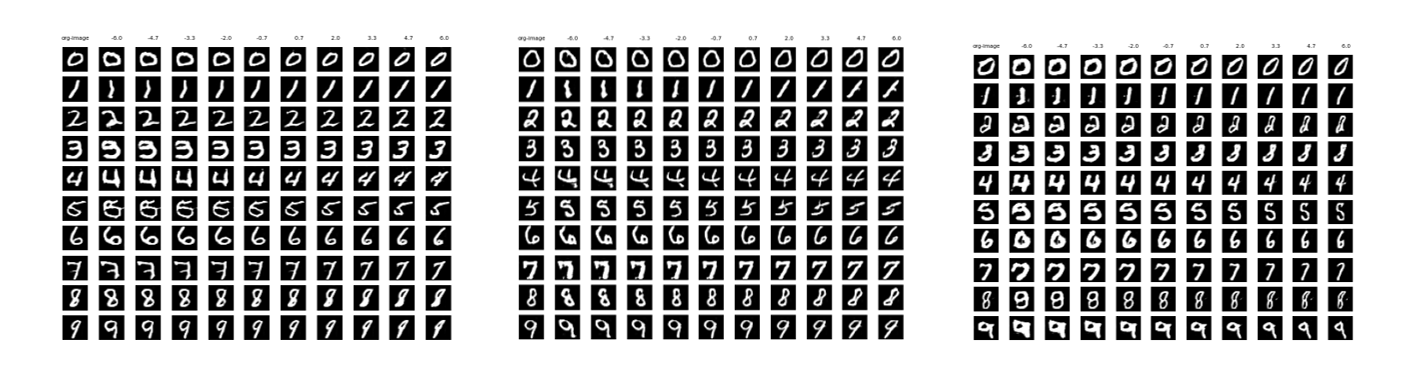
\includegraphics[scale=0.6]{cgan_d}
\caption{Discovered direction of CGAN on MNIST}
\label{fig:x cubed graph}
each bloch is the same direction, each row is a different seed generating all labels. Note how the latent space exclusively on the style - we can see changes in orientations and width.
\end{figure}

The latent space of CGAN seems to be much more 'organized' in the sense that it controls only the style of the digits and not their core characteristics. More over, the concepts of width and orientation, and even the size of the digit is reflected in the CGAN latent space. 



\subsection{Attention}

\begin{figure}[h]
\centering
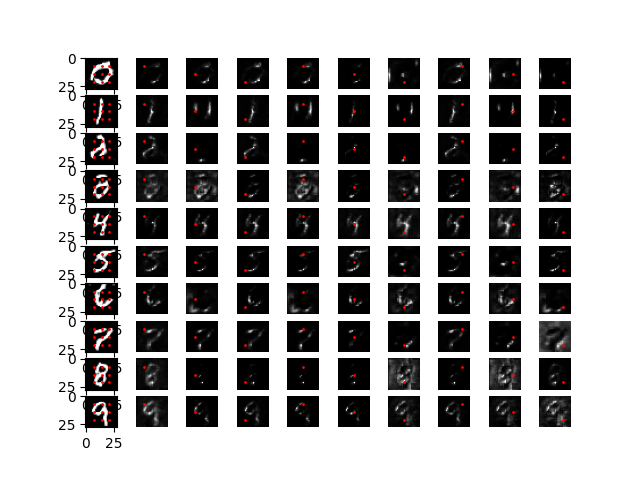
\includegraphics[scale=0.6]{attention_maps_gan}
\caption{attention maps of the generator model}
\label{fig:x cubed graph}
Leftmost image - the output image, with the location queries of the attention. each one of the images to the right is the attention map for that specific query - what areas of the previous layer the model pay attention to.
\end{figure}

Note that generally, the attention maps have the same general shape as the image generated. That means, that each pixel 'pays attention' to the whole generated image, and is activated based on that, and not just based on the features from the previous layer.
Another important insight so notice is that when the pixel we queried is silent, the maps seems to tend toward zero, while when the pixel is drawn, the maps reveal the main shape of the digit we draw.


\subsection{InfoGAN}


\subsubsection{Disentanglement representation}

Note that the InfoGAN generate different digits just by adjusting the input categorical code, but without any other enforcement as in CGAN (the embedding layer). The model is not aware to the different classes in the data, but still tend to do the 'right' separation in latent space, just by minimizing the information from that latent code to the images the generator produces. in the original paper it is mentioned that this classification by the categorical codes gets up to 95\% accuracy.


\begin{figure}[h]
\centering
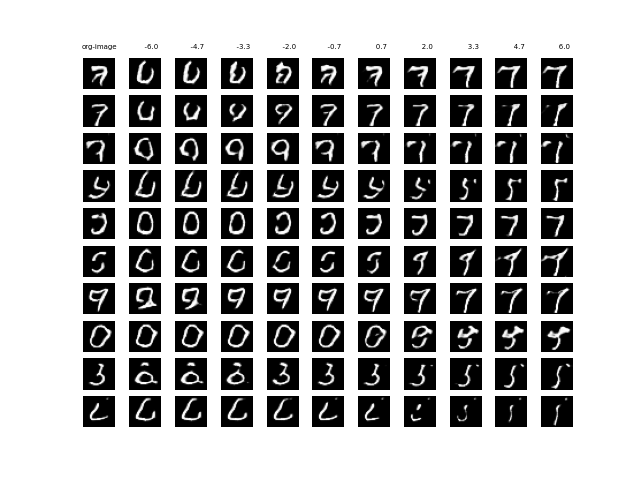
\includegraphics[scale=1]{gan_d1}
\caption{Discovered direction of GAN on MNIST}
\label{fig:x cubed graph}
\end{figure}




\section{ScrabbleGAN results}




\subsection{Directions in latent space}



\begin{figure}[h]
\centering
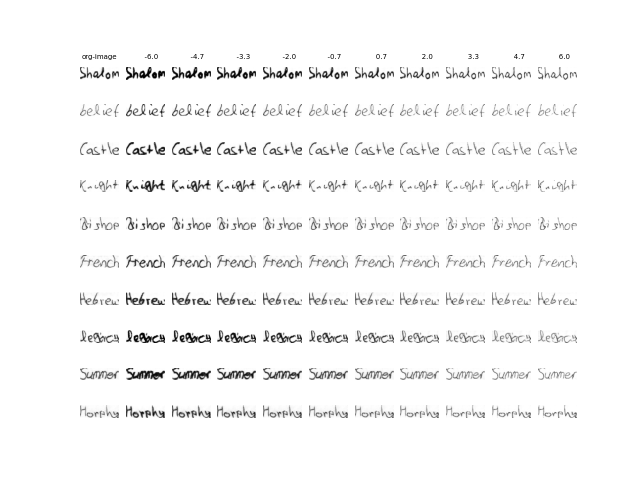
\includegraphics[scale=0.6]{Scrabble_d1}
\caption{Detected direction in ScrabbleGAN that effect the width of the writing}
\label{fig:x cubed graph}
\end{figure}

\begin{figure}[h]
\centering
\includegraphics[scale=0.6]{Scrabble_d2}
\caption{Detected direction in ScrabbleGAN that effect the cursivity of the writing}
\label{fig:x cubed graph}
\end{figure}


Though the algorithms was able to find direction that are meaningful to humans (Fig 6.9 and 6.10), it's still not as expressive as the one found in the MNIST GAN. That might relate to both the higher complexity of the problem (the change in R architecture might not be as optimal as possible), and also to the quality of the ScrabbleGAN generations.


\subsection{Attention}


\begin{figure}[h]
\centering
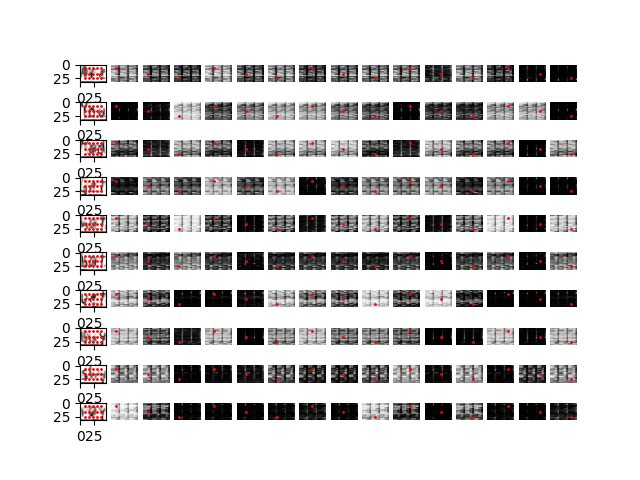
\includegraphics[scale=0.6]{Scrabble_attention}
\caption{ScrabbleGAN attention maps}
\label{fig:x cubed graph}
\end{figure}


Though we can find the same qualitative charactaristics in the attention maps of ScrabbleGAN output, they are much less informative and interpretable than in the MNIST case.
Note that as in MNIST data, queries where there is no writing seems to be silent (zero), and the one with writing are more activated.
Note the pattern that emerge in the map - it seems to be split by the number of characters, which obviously relates to the generation process. I would expect the maps to be more relevant, as in MNIST - to see shapes of the characters.


